
\documentclass[conference]{IEEEtran}
\usepackage{stmaryrd}
\usepackage{amsfonts}
% If the IEEEtran.cls has not been installed into the LaTeX system files,
% manually specify the path to it: e.g.,
% \documentclass[conference]{../sty/IEEEtran}

\usepackage{graphicx,times,amsmath} % Add all your packages here
\usepackage{epstopdf}
\usepackage{algorithm2e}
\usepackage{multirow}
\usepackage[hidelinks]{hyperref}
% correct bad hyphenation here
\hyphenation{op-tical net-works semi-conduc-tor IEEEtran}

\IEEEoverridecommandlockouts    % to create the author's affliation portion
                % using \thanks

\textwidth 178mm    % <------ These are the adjustments we made 10/18/2005
\textheight 239mm   % You may or may not need to adjust these numbers again
\oddsidemargin -7mm
\evensidemargin -7mm
\topmargin -6mm
\columnsep 5mm

\begin{document}


% paper title: Must keep \ \\ \LARGE\bf in it to leave enough margin.
\title{\ \\ \LARGE\bf Genetic Algorithm with Self-Adaptive Mutation Controlled by Chromosome Similarity\thanks{Daniel Smullen, Jonathan Gillett, Joseph Heron, and Shahryar Rahnamayan are with The Faculty of Engineering and Applied Science at the University of Ontario Institute of Technology, Oshawa, Ontario, Canada (email: \{daniel.smullen, jonathan.gillett, joseph.heron\}@uoit.net, shahryar.rahnamayan@uoit.ca).} \thanks{We would like to thank the SHARCNET organization for graciously providing the high performance computing facilities we needed to run our experiments.}}

\author{Daniel Smullen, Jonathan Gillett, Joseph Heron, Shahryar Rahnamayan}

% avoiding spaces at the end of the author lines is not a problem with
% conference papers because we don't use \thanks or \IEEEmembership
% use only for invited papers
%\specialpapernotice{(Invited Paper)}

% make the title area
\maketitle

\begin{abstract}
Proposed is a novel methodology for optimization of genetic algorithms using adaptive variable mutation. We replace the traditional mutation operator with an adaptive operator governed by population chromosome similarity. This approach is inspired from biological genetic expression which has increased incidences of genetic mutations as a result of `inbreeding' - we abstractly model this process as a fixed-size 1\% increase in mutation likelihood over generations, based on a static 15\% chromosome similarity threshold. Using combinatorial optimization with GA to solve the N-Queen problems, we determine optimal static mutation parameters for the traditional GA approach to use as a benchmark. We compare our approach to the benchmark for $N = 8$ through 32. Comparison between these optimized fixed mutation parameters and our adaptive variable approach shows better results using our approach for large problems ($N > 15$), with improving results for increasing values of N. A near tenfold increase in performance is yielded for $N = 32$.
\end{abstract}

% no key words

\section{Introduction}
\PARstart{G}{enetic algorithms} (GA) are particularly useful in areas which they can perform stochastic generation of solutions for combinatorial problems \cite{de1989using,crawford1992solving}. One well-known problem area includes the N-Queen problems. An efficient and common approach to solve these problems uses a genetic algorithms, encoding positions of queens into the chromsome. As with any genetic algorithm, evaluating the fitness of the chromosomes is required to determine the quality of candidate solutions \cite{srinivas1994genetic}, and only those with perfect fitness are solutions to the problem. 

Tuning up control parameters has a crucial effect on the GA's performance, which can increase or decrease based on the landscape and size of the problem encountered \cite{ye2010some,coyne1994genetic,srinivas1994adaptive}. We have found that by replacing traditional GA static mutation probability with a self-adaptive probability, better performance can be achieved when solving the N-Queen problems from both a single and multi-objective perspective, focusing on generating the most solutions possible within a fixed budget, and/or generating the first solution as quickly as possible. Our approach adapts based on the similarity of chromosomes in the population. The increase in performance is compounded in larger versions of the problem where the search space grows extremely large, such as the situation encountered when attempting to solve higher-order N-Queen problems. In this domain, deterministic methods prove useless.

Our solution approach was written in Java, and is available through GitHub under the \texttt{/gnu-user/genetic-algorithm-research} repository. It is licensed under the \textit{GNU General Public License, Version 3}.

\section{Background}
The N-Queen problems are multi-modal, with many local optima and global optima. 
Like many other complex optimization problems, the N-Queen problems become orders of magnitude larger as the number of queens and the size of the chessboard increases \cite{homaifar1992queens}. The problem is defined by the rules of chess and the protective embedded constraints of the chromosome which prevent queens from sharing rows or columns; when two queens share the same diagonal, a collision occurs, meaning that the board state is not a solution. A solution is found when all solutions have been found in which no queens on the board can attack another. This problem is {$O(n!)$} when approached using deterministic methods to find all possible solutions. Table {REFERENCE} shows the massive increase in problem size as $N$ increases. Further, it shows the proportionally huge increase in the number of distinct solutions. Based on the scale of the problem at higher values of $N$, using deterministic methods is too slow - the problem is simply too big. As $N$ increases, the problem becomes intractable. The number of distinct solutions for large values of $N$ is unknown, and the problem size becomes enormous. 

8-Queen is the classical version of N-Queen. The histogram found in Figure {REFERENCE} shows the full deterministic traversal of the 8-Queen problem landscape, which is characteristic of the N-Queen problems. It details the myriad possibilities for the number of board states which can occur even in a relatively small problem size. Not pictured in this figure are the 4 instances of 44 simultaneous collisions, and 2 instances of 56 collisions. These occur when 7 of 8, or all 8 queens are all placed on the diagonal respectively. 

While finding the most solutions given a fixed number of function calls (GA generations) was the main objective of our proposed approach, fundamentally there are two objectives in N-Queen problems; finding the first solution as fast as possible is an alternative objective. The latter problem can be solved in polynomial time through conventional means.

\section{Related Work}
Deterministic attempts to solve N-Queen problems have been made successfully only for values of $N$ up to 26, and attempts to find single solutions quickly have been made for versions of the problem up to {$N = 500000$}. There are no known integer sequences or proofs which can represent the number of distinct solutions for $N > 26$, nor is there a deterministic means which can find them all within human time frames.

Since tuning control parameters has a profound effect on the evaluation of GA, one might conclude that there is an optimal static mutation probability for solving N-Queen problems. Hesser and M\"{a}nner [CITE] attempted to find such a value for GA in general but failed - there is no perfect algorithm, and it is rare that there is an optimal control parameter for a very good algorithm which fits all circumstances. This is an important axiom of the No Free Lunch (NFL) theorem. Finding the pragmatic best case scenario for static mutation probabilities ({REFERENCE SYMBOL}) within traditional GA proved to be a useful control and benchmark for our experiments, as can be seen in our results.

Other alternative approaches to enhancing GA for combinatorial optimization sought to increase population diversity in order to overcome wasteful convergence on local optima, which is problematic in N-Queen since it has many local and global optima. Combining standard GA with randomly generated individuals into the population is well studied[CITE], but fails to adapt to suit the problem. Still, exploring the nature of genetic diversity provides valuable insight into the motivation for increasing diversity among candidate solution populations to reach better solutions.

Adaptive approaches have historically manipulated GA control parameters by changing the mutation probability over time [CITE] such that it is low during exploration, high during exploitation, or vice-versa. Other approaches used the overall mean population fitness to adjust genetic operators[CITE]. Alternative adaptive approaches changed mutation probabilities between two values based on fitness [CITE], while others attempted to individually specify genetic operator probabilities into the phenotype, encoded with meta-operators that govern them [CITE]. All adaptive approaches sought to yield more fruitful explorations of the problem landscape by tuning GA control parameters, but most approaches have been limited by being na\"{i}ve to problem size or the state of exploration and diversity. These methodologies, however, yield many advantages over traditional GA in that they preclude the need for \textit{a priori} knowledge about optimal control parameters, mitigating the need to 'tune them up' with protracted test runs prior to long-term evaluation.

\section{Proposed Approach}\label{params}
Our main motivation for this new self-adaptive approach was to emulate the observed tendency in nature for mutations to occur as a result of inbreeding [CITE]. Our desire was to replicate this behavior with GA in with the idea that inbreeding driven mutations increase genetic diversity in animals (for better or for worse). Therefore, it stood to reason that a similar phenomenon might occur in GA. Exploring this idea yielded surprising results.

We used a GA with an integer encoded chromosome to represent the N-Queen positions on the chessboard. By limiting queens to single rows and columns, our approach includes protective embedded constraints. It uses traditional GA operators - selection, mutation, and recombination. Ordinary roulette wheel selection is used in conjunction with single-point crossover and single-value uniform mutation. 

Chromosome similarity is used as the defining characteristic of our adaptation approach. The probability for the mutation operator is variable, while recombination ({REFERENCE SYMBOL}) remains at a single static value as in traditional GA. The mutation operator probability delta (per 1 generation) is set to a fixed value. Our experimental values for the genetic operators are seen in Table {REFERENCE}. 

\subsection{Self-Adaptive Mutation}
In order to apply our self-adaptive mutation approach, a two step process is required. For each generation of chromosomes, the population's chromosome similarity must be evaluated. The similarity algorithm is detailed in Algorithm \ref{alg:similarity}.  

When the chromosome similarity is less than the specified threshold ({REFERENCE SYMBOL}), the population is too dissimilar. This means the mutation probability must decrease, because the population is not inbred. For the next generation, the mutation probability is subtracted by the fixed delta value seen in Table {REFERENCE}. After genetic operations and selection the next generation is populated and their chromosome similarity is calculated. If the chromosome similarity has increased again, and it is above the specified threshold, the population is inbred. {REFERENCE SYMBOL} must increase by the fixed delta in the next generation.

Variations in chromosome similarity may result independently of uniform mutation. Since the recombination probability is 70\%, the resultant permutations of the genome are likely to be approximately 30\% similar (due to cloning) unless uniform mutation has occurred on cloned genes. The observed result using adaptive mutation is that the chromosome similarity will approach an equilibrium percentage approximately equal to the specified similarity threshold as generations evolve.

\subsection{Chromosome Similarity Algorithm}
Chromosome similarity is calculated using a greedy algorithm, seen in Algorithm \ref{alg:similarity}. First, the chromosomes' genes are decoded and re-encoded into integer values and concatenated into one large integer value. Next, the resultant array of integer representations is sorted. Our implementation uses the quick-sort algorithm provided by Java for minimal computational overhead. This gives the similarity algorithm its' characteristic asymptotic behavior, as the complexity of the sorting function itself is of higher complexity than the rest of the main similarity calculation algorithm. Quick-sort runs on average in $O(n \log n)$ complexity, although it should be noted that in the theoretical worst case, quick-sort works in $O(n^2)$ which is highly unlikely. The main algorithm runs in $O(n)$ linear complexity independent of the sorting. Similar chromosomes have the same genes. A population with 100\% similarity is completely identical.

\begin{algorithm}
  \SetKwProg{Fn}{Function}{}{end}\SetKwFunction{Similarity}{Similarity}%
  \SetKwData{Similar}{similar}\SetKwData{Value}{value}\SetKwData{Matched}{matched}\SetKwData{Length}{length}\SetKwArray{Sorted}{sorted}
  \SetKwFunction{Sort}{Sort}
  \SetKwInOut{Input}{input}\SetKwInOut{Output}{output}
  \SetAlgoLined
  \DontPrintSemicolon
  
  \Fn{\Similarity{$chromosomes$}}{
  
  \Input{An array of $chromosomes$}
  \Output{Fraction of chromosomes that are similar}
  \BlankLine
  
  \Similar $\leftarrow$ 0\;
  \Matched $\leftarrow$ false\;
  \Length $\leftarrow$ length of $chromosomes$\;
  \BlankLine
  
  \tcp{Sort using an arbitrary sorting algorithm}
  \Sorted $\leftarrow$ \Sort{$chromosomes$}\;
  \BlankLine
  
  \For{$i \leftarrow 0$ \KwTo $\Length -1$}
  {
    \uIf{\Sorted{$i$} == \Sorted{$i + 1$}}
    {
      \Similar $\leftarrow$ \Similar + 1\;
      \Matched $\leftarrow$ true\;
    }
    \ElseIf{\Matched}
    {
      \Similar $\leftarrow$ \Similar + 1\;
      \Matched $\leftarrow$ false\;
    }
    \BlankLine
    
    \tcp{Case where the last item is a match}
    \If{\Matched and $\left(i + 1 == \Length - 1 \right)$}
    {
      \Similar $\leftarrow$ \Similar + 1\;
    }
  }
  \BlankLine
  \KwRet{\Similar / \Length}
  }
\caption{Chromosome similarity function}
\label{alg:similarity}
\end{algorithm}

\subsection{Fitness Function}
Candidate solution fitness is evaluated by determining the number of collisions between queens on the chessboard. This means that in a board state where one queen can attack another, two collisions result. The algorithm for determining the fitness of a given board state is given in Algorithm \ref{alg:fitness}, showing the mechanisms used to find collisions across diagonals on the board. The overall board state fitness is calculated as $fitness = \frac{1}{C}$, where $fitness = 1$ if $C = 0$. The number of collisions is $C$. Maximum fitness is achieved when $C = 0$ as there are no collisions, resulting in a distinct board solution.
 
\begin{algorithm}[t!]
  \SetKwProg{Fn}{Function}{}{end}\SetKwFunction{Fitness}{Fitness}%
  \SetKwData{Collisions}{collisions}\SetKwData{Length}{length}\SetKwArray{Chromosome}{$chromosome$}\SetKwData{Yi}{$y_i$}\SetKwData{Yj}{$y_j$}
  \SetKwFunction{Abs}{abs}
  \SetKwInOut{Input}{input}\SetKwInOut{Output}{output}
  \SetAlgoLined
  \DontPrintSemicolon
  
  \Fn{\Fitness{$chromosome$}}
  {
    \Input{A single $chromosome$}
    \Output{A fitness value for the chromosome}
    \BlankLine
    
    \Collisions $\leftarrow$ 0\;
    \Length $\leftarrow$ length of the $chromosome$\;
    \BlankLine
    
    \For{$i \leftarrow 0$ \KwTo $\Length -1$}
    {
      \tcp{Check each gene against the current}
      $j \leftarrow \left( i + 1 \right) \mod{\Length}$\;
      \While{$j$ != $i$}
      {
        \Yi $\leftarrow \Chromosome{i}$\;
        \Yj $\leftarrow \Chromosome{j}$\;
        \BlankLine
        
        \tcp{Check for vertical collision}
        \If{\Yi == \Yj}
        {
          \Collisions $\leftarrow \Collisions + 1$\; 
        }
        \BlankLine
        
        \tcp{Check for diagonal collision}
        \If{\Abs{$\left(i - j \right)$ / $\left(\Yi - \Yj \right)$} == 1}
        {
          \Collisions $\leftarrow \Collisions + 1$\;
        }
        \BlankLine
        
        $j \leftarrow j + 1$\;
        $j \leftarrow j \mod{\Length}$\;
      }
    }
    \BlankLine

    \eIf{\Collisions == 0}
    {
      \KwRet{1}\;
    }
    {
      \KwRet{1 / \Collisions}\;
    }
  }
\caption{Fitness function}
\label{alg:fitness}
\end{algorithm}

\subsection{Identifying Distinct Solutions}
Each generation, there is a likelihood that some of the chromosomes in the current population are valid solutions - any of the current generation's chromosomes with a fitness of 1 is some sort of solution. Whether it is distinct or not is unknown at first. When a solution is found, it must be compared to the list of previously found solutions. Each generation, there is always a strong possibility that many candidate solutions are duplicates of previously found solutions. Symmetry operations are applied to each solution found to generate more distinct solutions based on the symmetrical nature of the chessboard. This may further increase the likelihood that the new population's solutions have already been found previously. Therefore, indistinct solutions are discarded without having symmetry operations applied as their reconfiguration would already be identical to symmetric configurations of previously found distinct solutions. After saving newly found solutions, the new generation replaces the previous generation and the GA continues.

Symmetry operations consist of three $90^{\circ}$ rotations, a horizontal reflection, and then 3 further $90^{\circ}$ rotations of the reflected board. Each symmetrical board configuration is a candidate solution that is checked against the existing distinct solution, and discarded if it has already been found previously. Each distinct solution can potentially yield 8 more distinct solutions depending on the placement of queens.

\section{Experimental Methodology}
We measured the performance of our self-adaptive approach using an empirical study. Our methodology was to solve N-Queen problems for various values of N with a limited budget of function calls (generations), repeated a multitude of times to ensure accuracy and collect aggregate statistics. Table {REFERENCE} shows the number of function calls permitted and the number of trials run for each value of N. Special budgets and trial multiplicities were set for $N = 32$ in order to accommodate the exceptionally large problem size.

Our control used traditional GA with fixed mutation probabilities ({REFERENCE SYMBOL Mc}) of {SYMBOL} = 1\%, 5\%, 10\%, 15\%, 20\%, 25\%, 30\%, 35\%, 40\%, 45\%, 50\%, 55\%, 60\%, 65\%, 70\%, 75\%, 80\%, 85\%, 90\%, 95\% and 100\% to solve each N-Queen problem. These trials were run with the same multiplicity and budget as our self-adaptive approach. The goal of the control trials was to approximately determine the optimal {REFERENCE SYMBOL Mc} for finding the most solutions for each problem given the budget, and finding the first solution in as few generations as possible. Our aim was to test our new approach against a reasonable approximation of the best possible performance that the traditional GA approach can provide. Optimized control parameters for mutation would be determined and used as a benchmark, similar to Hesser and M\"{a}nner's study.

For $N = 8$ through 16, 30 tests were performed at each {REFERENCE SYMBOL Mc} ($21 \times 30 = 630$ tests total), and 30 runs were performed using the self-adaptive approach. For $N = 18$ through 26, 15 tests were performed. For $N = 32$, 10 tests were performed. Given the increasingly large problem sizes, the number of tests were reduced in order to allow experimentation to complete within reasonable human time frames. Descriptive statistics were gathered every 1000 generations, with means calculated using the grand mean.

\section{Results and Analysis}
It became clear very quickly when we plotted the results of our tests that the variable mutation method was not suitable in its current configuration for the simpler N-Queen problems. In fact, we found that given sufficient knowledge about the problem landscape for the lower-order problems, the right static mutation value would likely beat variable mutation every time. However, for ordinary non-benchmark usage of genetic algorithms it is useless to use a static mutation rate value unless you already know the best mutation rate for the problem. This generally speaks to the point that having an adaptive mutation rate approach will likely find this value. The smaller N-Queen problems are too small to merit the usage of a stochastic approach regardless, as deterministic methods can yield solutions quickly with guaranteed success.

\subsection{Traversing the Problem Landscape}
Moving into more complex and larger problems is where the adaptive mutation approach becomes increasingly successful. Our reasoning is that this may have something to do with the similarity threshold value that was chosen (15\%). Further tuning of this parameter may yield better results for larger or smaller problems. We have created a conceptual model for our findings which may yet be validated in future studies.

Mapping the stochastic solution landscapes for the N-Queen problems means plotting a random non-deterministic traversal of the solution space to a linear axis. Each sequential value on this axis corresponds to each integer sequence of solutions encoded in the chromosomes. A linear traversal of this landscape implies a uniformly random traversal of the randomly generated solutions. This plot, in contrast to the deterministic solution space yielded by consecutively plotting the values of the integer encoded chromosome, shows very few similarities. There is no way to plot a random traversal except by noting that as time approaches infinity, all solutions will have been traversed and the full contour of the landscape will be visible. This could just as easily be yielded by a consecutive linear traversal, but the point of using GA rather than a deterministic traversal is that GA makes the traversal 'smarter' by searching for values which have better fitness, attracted toward fitness peaks\cite{srinivas1994genetic}. The mutation operator helps to prevent the current position in the traversal from being stuck in a local optimum \cite{ye2010some}. It provides an extra impulse to shift position further towards what a potential solution, and away from previously traversed areas of the landscape.

Given this knowledge, assuming a linear traversal of this random axis is possible in one given test, we can evaluate the characteristics of each GA mutation parameter configuration and map them to this conceptual model. The starting point on the plot is a random location on the landscape. From there, the next location is likely to be within a radius of probable new chromosomes surrounding this area. We have come to refer to this radius of probable chromosomes as the 'step size', and we believe there is some relationship between the step size and the fixed mutation rate. The fixed mutation rate governs the maximum distance from the current position in the traversal to the furthest step away. What this means for solution landscapes like that of the N-Queen problems is that all solutions which are close to the intersections of these steps are easier to find because there is a greater total probability of landing within their vicinity. Solutions which are clustered very close together on this random landscape, however, will likely be stepped around for several generations before convergence on the actual solution occurs.

The variable mutation rate's adaptive nature allows for this fixed step size to be ignored because it introduces the ability to vary the step size when convergence upon a solution occurs. The result is that the probability distribution over the entire solution landscape is more uniformly smaller away from solutions, and larger within the vicinity of solutions. Our reasoning is that if the static mutation rates have a fixed step size, the variable mutation rate does not, and adaptation will vary the step size so as to maintain the chromosome similarity. Further, this decreases the likelihood of overshooting a solution and having to step back around again, because the variability of the mutation rate allows for smaller or larger steps when needed.

In general, this conceptual model will require extensive further study to validate it's correctness. Meanwhile, the empirical evidence presented in our plotted results shows the validity of our adaptive mutation approach.

\subsection{Plotted Results and Observations}
Figure \ref{fig:best_solution_all_queens} depicts the best fixed mutation rate, that found the most solutions for each problem size, versus the variable mutation rate. Each of these plots are cut off at 10 million generations. In spite of the fact that the 32-Queens problem was allowed to run up to 50 million generations, we are only showing plots which are trimmed to this value for consistency of comparison. The plots show that as the problem size increases from the smaller problems up to 14 queens, the fixed mutation rates reach peak performance. In these problems, the most optimal fixed mutation rate is better than the variable mutation rate. This trend changes at the 15 queens where they are nearly equal. From there on, the difference in performance becomes significant - variable mutation consistently finds more solutions than the most optimal fixed mutation rate. 

The optimal fixed mutation rate decrease from 95\% for 8 queens down to 65\% for 32 queens. As the problem size increases, we observe that this trend continues. This can be seen in Table \ref{table:mostsol}. From 15 queens up to 32 queens, there is a divergence between the performance of fixed mutation and variable mutation. A steep decline is visible in the performance of the best fixed mutation rates as the problem size increases. The performance of the variable mutation rate also decreases with increased problem sizes, but at a far lesser rate. This marginal decrease in performance yields the conclusion that variable adaptive mutation rates will perform far better for larger problems.

An interesting result was observed when viewing the box plots showing the range of chromosome similarity values for each static mutation rate. We found that whenever the similarity has the greatest inter-quartile range (IQR), the corresponding static mutation rate performed best. This contributed heavily to the step size concept we believe is exhibited by the system. We also found that as the problem landscape grows larger in higher order N-Queen problems, the IQR decreases in size. There is a possibility that the IQR will decrease towards convergence on a single value in higher order problems, which suggests that there may be a pattern to the convergence which can be approximated and leveraged for predicting optimal static mutation rates for any N-Queen problems. In the 14-Queens problem, the IQR was approximately 20\%. In the 32-Queens problem, the IQR was approximately 3\%. Since testing this requires exhaustive experimentation in order to definitively find the optimal static mutation rate for any given problem, this further supports the notion that a variable mutation rate is a more practical approach. As shown prominently in Figure \ref{fig:fitness_all_mutation_14}, we have found that the relationship between the best fixed mutation rates and the largest IQR is visible. The fixed mutation rate of 80\% clearly has the largest IQR, and correspondingly the most number of solutions found. This trend is visible for all values of N in the N-Queen problems. 

However, when approaching problem sizes of $N > 14$, the observation no longer holds true - adaptive variable mutation rates are consistently better, but have comparatively similar IQR to the worse performing static mutation rates. We noticed a new relationship here, showing that the IQR of the variable mutation rate is closest to the trend followed by the IQR of the increasing static mutation rates. There is a sharp drop-off, however, immediately upon reaching the best static mutation rates within this trend. This supports the step-size concept in that we can see the inability of the static mutation rate to converge upon the most desirable fitness values. There is a clear convergence on this value with the adaptive mutation rate, consistently approaching the 25\% fitness value. The most optimal static mutation rate in our experimentation is higher than the true optimum, resulting in a sharp falloff of fitness values. In Figure \ref{fig:best_solution_all_queens}, the 14-Queens problem shows the best static mutation rate is 80\%, which performs substantially better than any other static mutation rate. In Figure \ref{fig:fitness_all_mutation_14}, this static mutation clearly has the largest IQR. In the 32-Queens problem, the 65\% fixed mutation rate is the best performer, but is beaten nearly tenfold in performance by the variable mutation rate.

Figure \ref{fig:mutation_rate_all_queens} shows a box plot with an overlaid trend line. The box plots in this figure show the IQR for the mutation rate of the variable adaptive method. The points show the best performing static mutation rate for each N-Queen problem. This plot shows the convergence trend of the IQR in the variable mutation rates as the problem size increases. There is also a trend that shows the best performing static mutation rates decrease as the problem size increases. Where the trend and the box plots intersect at the 15-Queens problem, we can see in the corresponding Figure \ref{fig:best_solution_all_queens} that the performance is nearly the same.


%%%%%%%%%%%%%%%%%%%%%%%%%%%%%%%%%%%%%%%%%%%%%%%%%%%%%%%%%%%%%%%%%
% 
% TABLES
%
%%%%%%%%%%%%%%%%%%%%%%%%%%%%%%%%%%%%%%%%%%%%%%%%%%%%%%%%%%%%%%%%%
\begin{table}
\centering
\caption{N-Queen Problems Distinct Solutions}
\begin{tabular}{|l|l|l|} \hline
N  & Problem Size (N!)      & Distinct Solutions      \\ \hline
8  & 40320                      & 92                     \\
9  & 362880                     & 352                    \\
10 & 3628800                    & 724                    \\
11 & 39916800                   & 2680                   \\
12 & 479001600                  & 14,200                 \\
13 & 6227020800                 & 73,712                 \\
14 & 87178291200                & 365,596                \\
15 & $1.307674368\times10^{12}$ & 2,279,184              \\
16 & $2.092278989\times10^{13}$ & 14,772,512             \\
17 & $3.556874281\times10^{14}$ & 95,815,104             \\
18 & $6.402373706\times10^{15}$ & 666,090,624            \\
19 & $1.216451004\times10^{17}$ & 4,968,057,848          \\
20 & $2.432902008\times10^{18}$ & 39,029,188,884         \\
21 & $5.109094217\times10^{19}$ & 314,666,222,712        \\
22 & $1.124000728\times10^{21}$ & 2,691,008,701,644      \\
23 & $2.585201674\times10^{22}$ & 24,233,937,684,440     \\
24 & $6.204484017\times10^{23}$ & 227,514,171,973,736    \\
25 & $1.551121004\times10^{25}$ & 2,207,893,435,808,352  \\
26 & $4.032914611\times10^{26}$ & 22,317,699,616,364,044 \\
\dots & \dots & Unknown				\\
\hline\end{tabular}
\label{table:numuniquesol}
\end{table}

\begin{table}
\centering
\caption{Most N-Queens Distinct Solutions}
\begin{tabular}{|l|l|l|} \hline
N&               Mutation Rate&  Distinct Solutions\\ \hline
\multirow{2}{*}{8}&   0.95&           92\\
&                     variable&       92\\ \hline
\multirow{2}{*}{9}&   0.95&           352\\
&                     variable&       352\\ \hline
\multirow{2}{*}{10}&  0.9&            724\\
&                     variable&       724\\ \hline
\multirow{2}{*}{11}&  0.85&           2,680\\
&                     variable&       2,680\\ \hline
\multirow{2}{*}{12}&  0.85&           13,690\\
&                     variable&       11,986\\ \hline
\multirow{2}{*}{13}&  0.8&            32,128\\
&                     variable&       26,308\\ \hline
\multirow{2}{*}{14}&  0.8&            41,520\\
&                     variable&       29,520\\ \hline
\multirow{2}{*}{15}&  0.8&            30,356\\
&                     variable&       30,324\\ \hline
\multirow{2}{*}{16}&  0.8&            15,016\\
&                     variable&       30,132\\ \hline
\multirow{2}{*}{18}&  0.75&           16,392\\
&                     variable&       27,120\\ \hline
\multirow{2}{*}{20}&  0.75&           7,872\\
&                     variable&       25,608\\ \hline
\multirow{2}{*}{22}&  0.7&            6,008\\
&                     variable&       25,376\\ \hline
\multirow{2}{*}{24}&  0.7&            6,440\\
&                     variable&       24,560\\ \hline
\multirow{2}{*}{26}&  0.7&            6,280\\
&                     variable&       23,008\\ \hline
\multirow{2}{*}{32}&  0.65&           15,216\\
&                     variable&       104,080\\
\hline\end{tabular}
\label{table:mostsol}
\end{table}


\begin{table}
\centering
\caption{First N-Queens Distinct Solution}
\begin{tabular}{|l|l|l|l|} \hline
N&          Best $M_{c}$&  $\mu$ Generations $M_{c}$&  $\mu$ Generations $M_{a}$\\ \hline
 8&         0.75&             45&                 91\\ \hline
 9&          0.8&            121&                186\\ \hline
10&          0.8&            261&                417\\ \hline
11&          0.7&            444&                364\\ \hline
12&         0.65&            457&                463\\ \hline
13&          0.7&            448&                582\\ \hline
14&         0.65&            494&                609\\ \hline
15&         0.65&            598&                513\\ \hline
16&         0.65&            662&                606\\ \hline
18&         0.65&            911&                688\\ \hline
20&         0.55&            889&                862\\ \hline
22&          0.5&           1234&               1211\\ \hline
24&          0.4&           1209&               1182\\ \hline
26&         0.45&           1599&                942\\ \hline
32&          0.5&           2298&               1995\\ \hline
\end{tabular}
\label{table:firstsol}
\end{table}




%%%%%%%%%%%%%%%%%%%%%%%%%%%%%%%%%%%%%%%%%%%%%%%%%%%%%%%%%%%%%%%%%
% 
% FIGURES
%
%%%%%%%%%%%%%%%%%%%%%%%%%%%%%%%%%%%%%%%%%%%%%%%%%%%%%%%%%%%%%%%%%
\begin{figure}
\centering
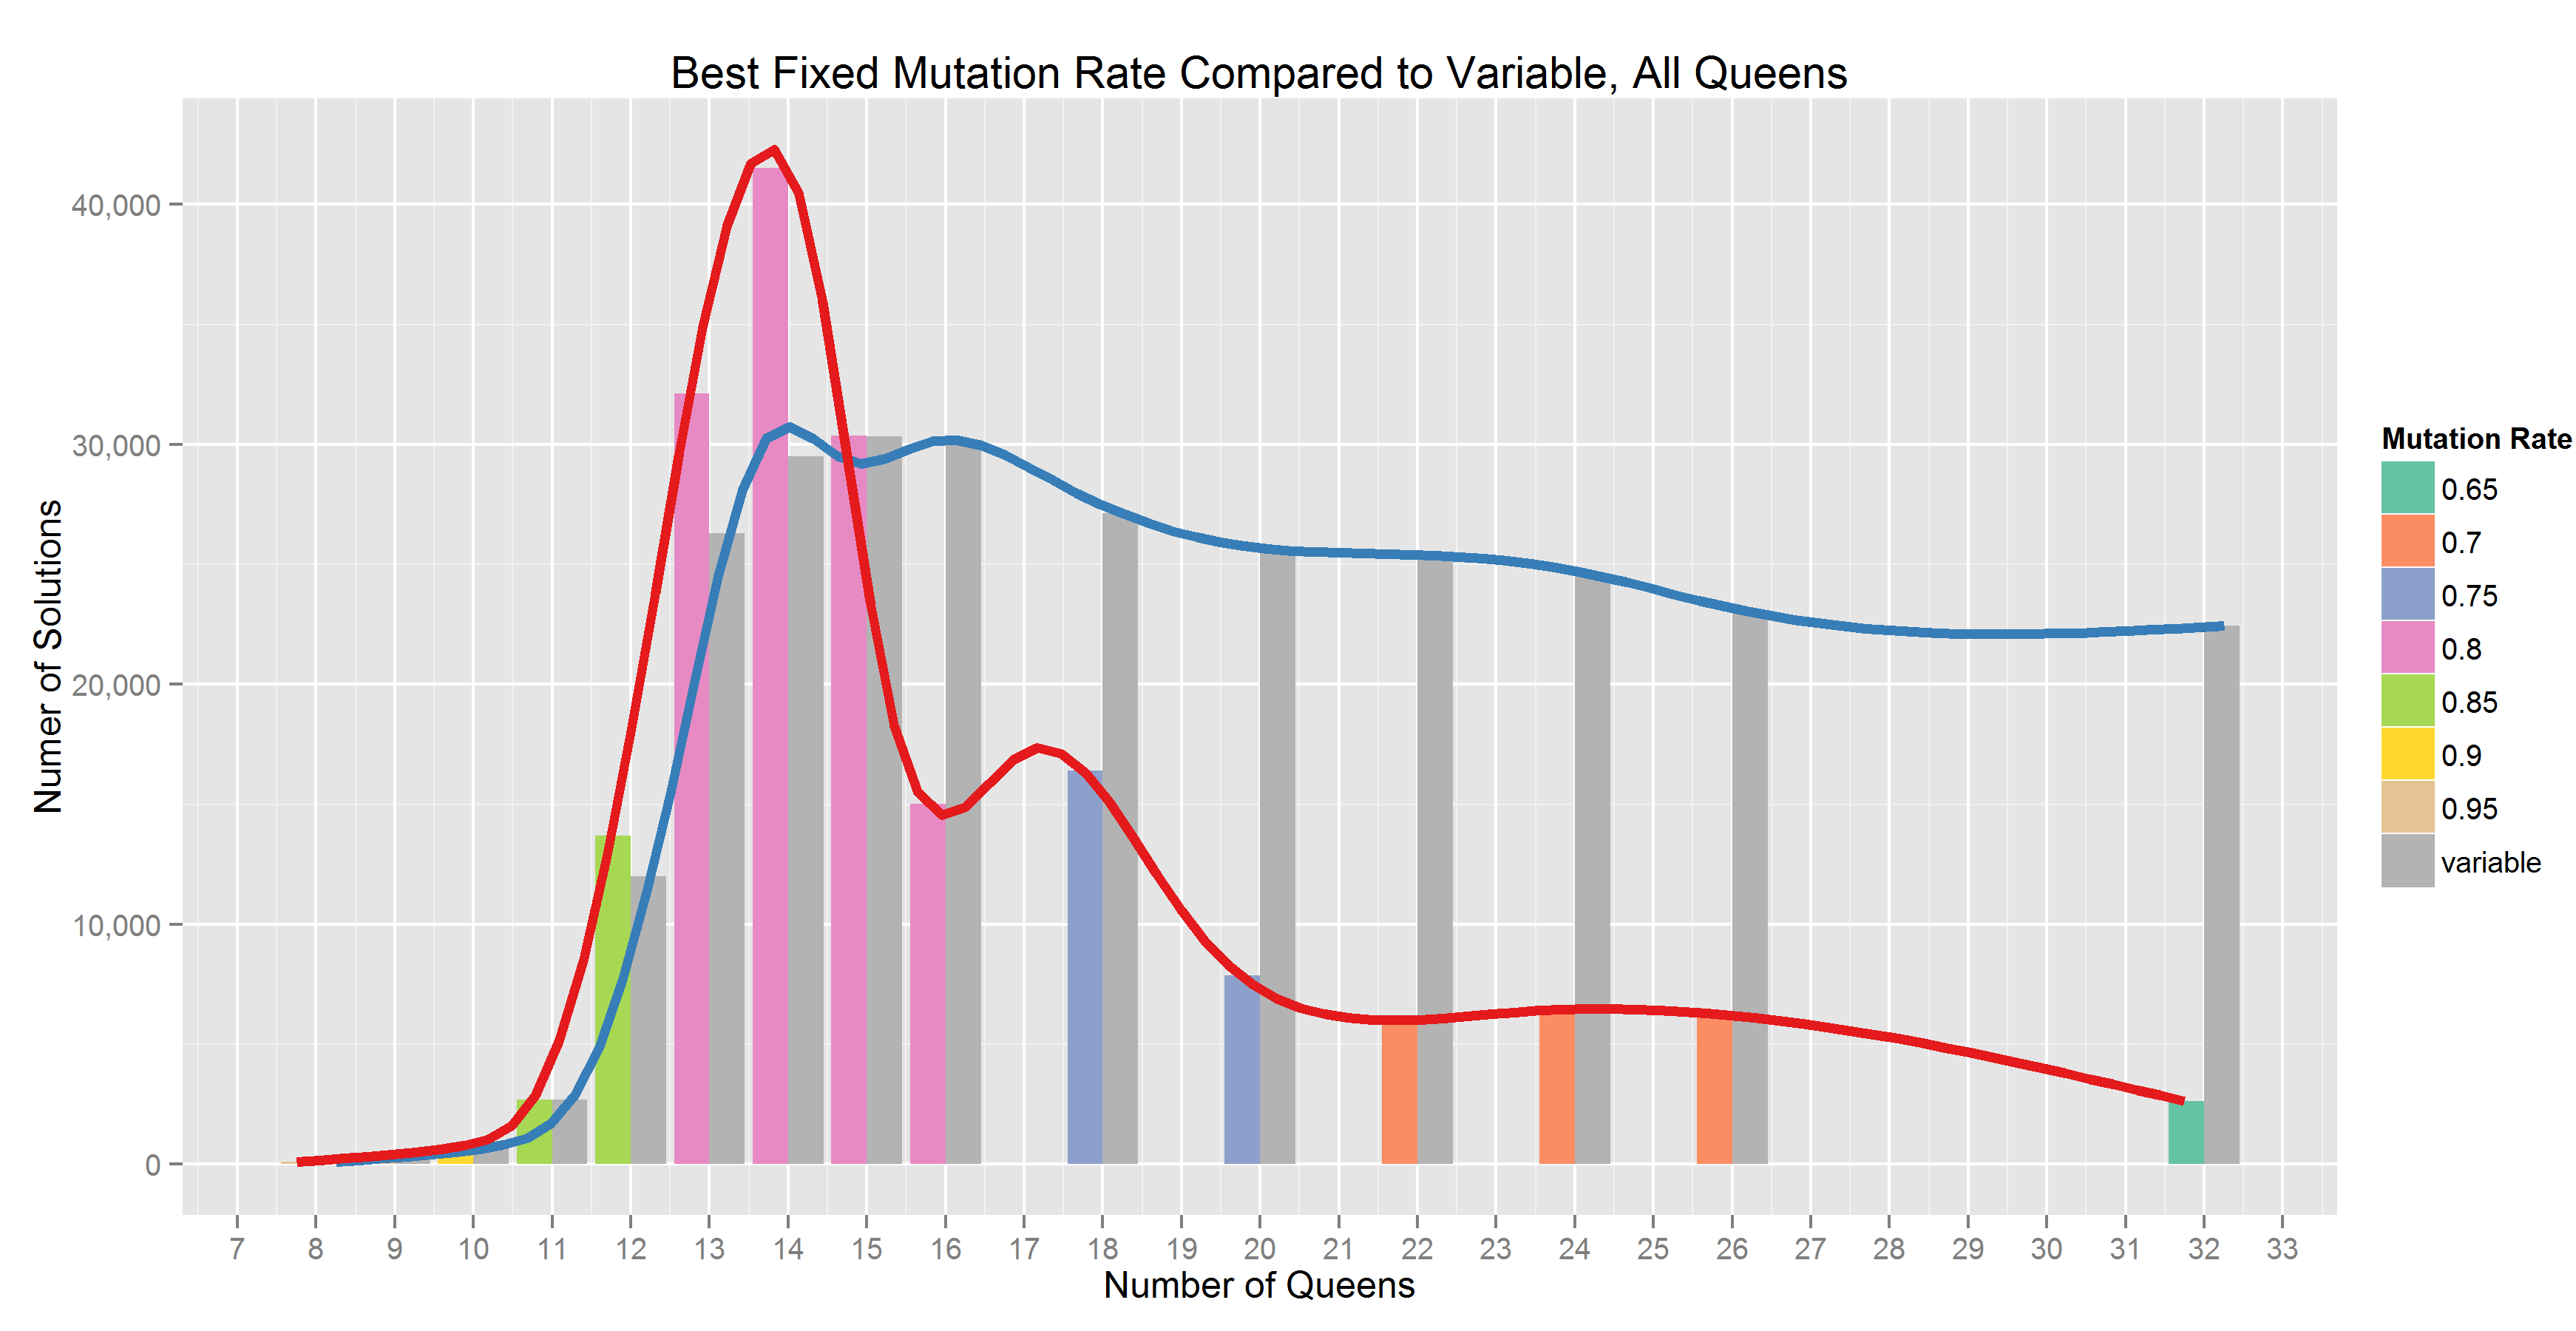
\includegraphics[width=0.50\textwidth]{best_solution_all_queens.png}
\vspace{-18pt}
\caption{Best Fixed and Variable Mutation Solutions}
\label{fig:best_solution_all_queens}
\end{figure}

\begin{figure}
\centering
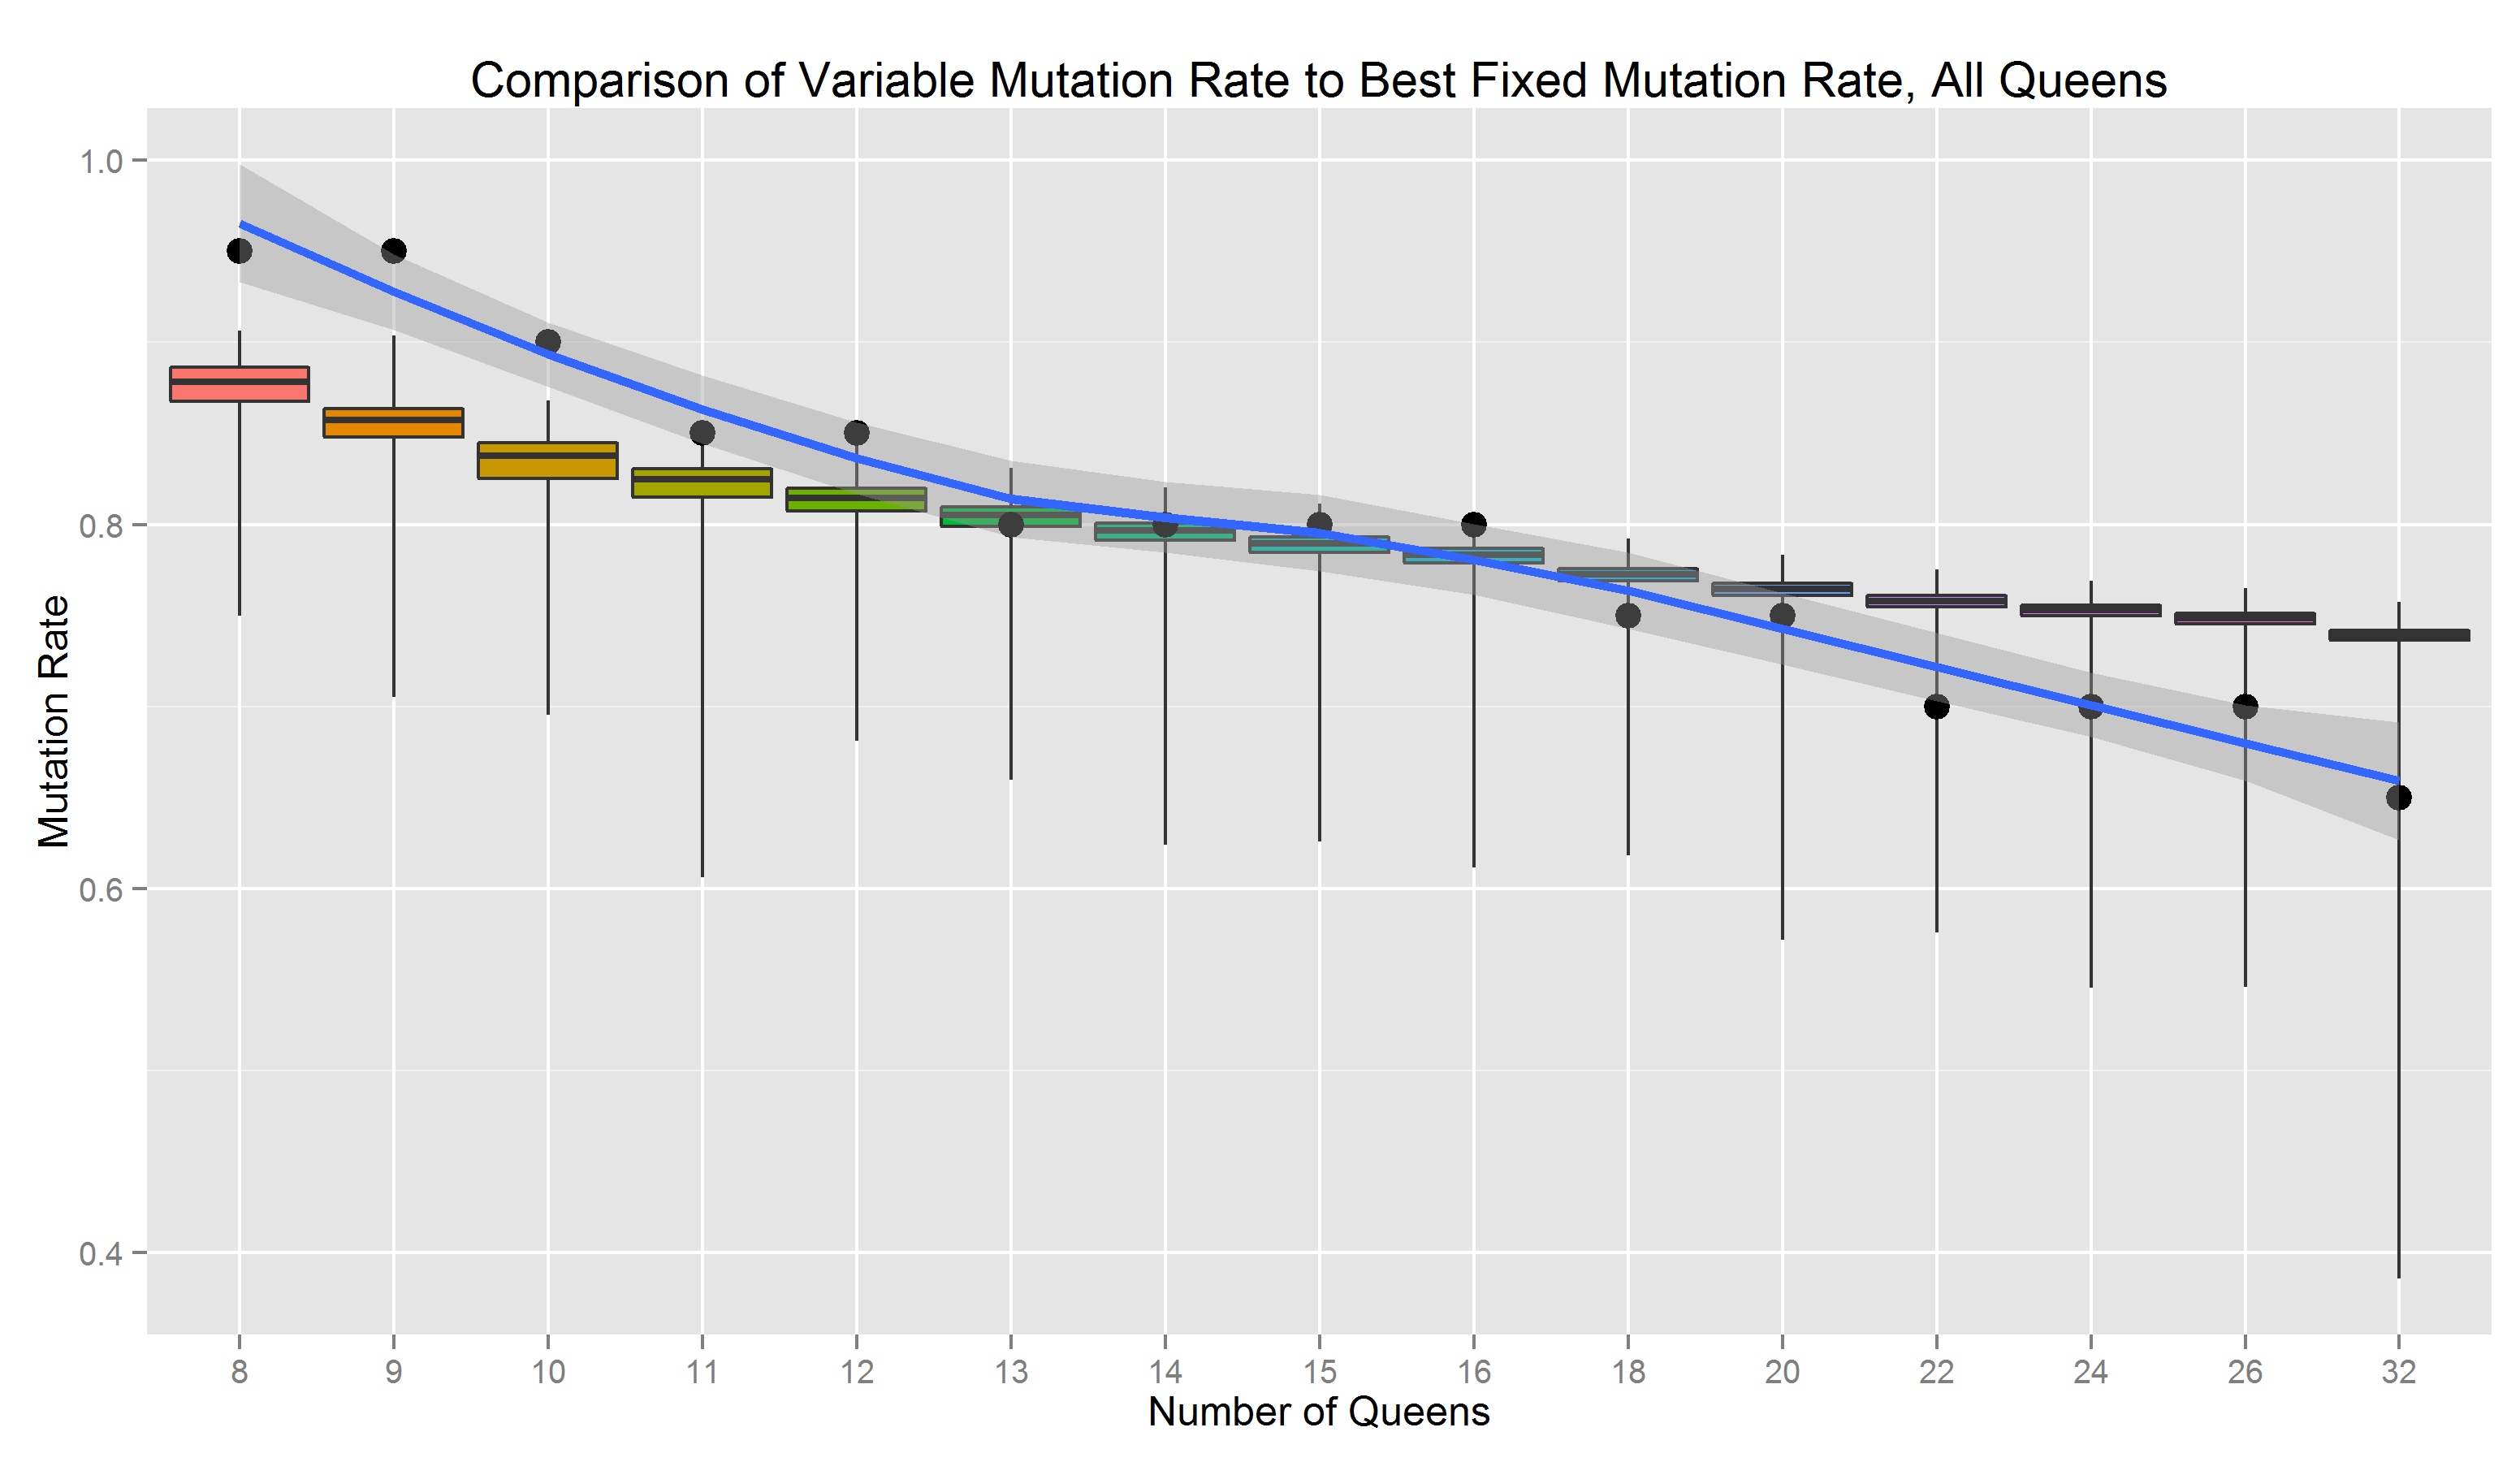
\includegraphics[width=0.50\textwidth]{mutation_rate_all_queens.png}
\vspace{-18pt}
\caption{Best Fixed and Variable Mutation Rates}
\label{fig:mutation_rate_all_queens}
\end{figure}

\begin{figure}
\centering
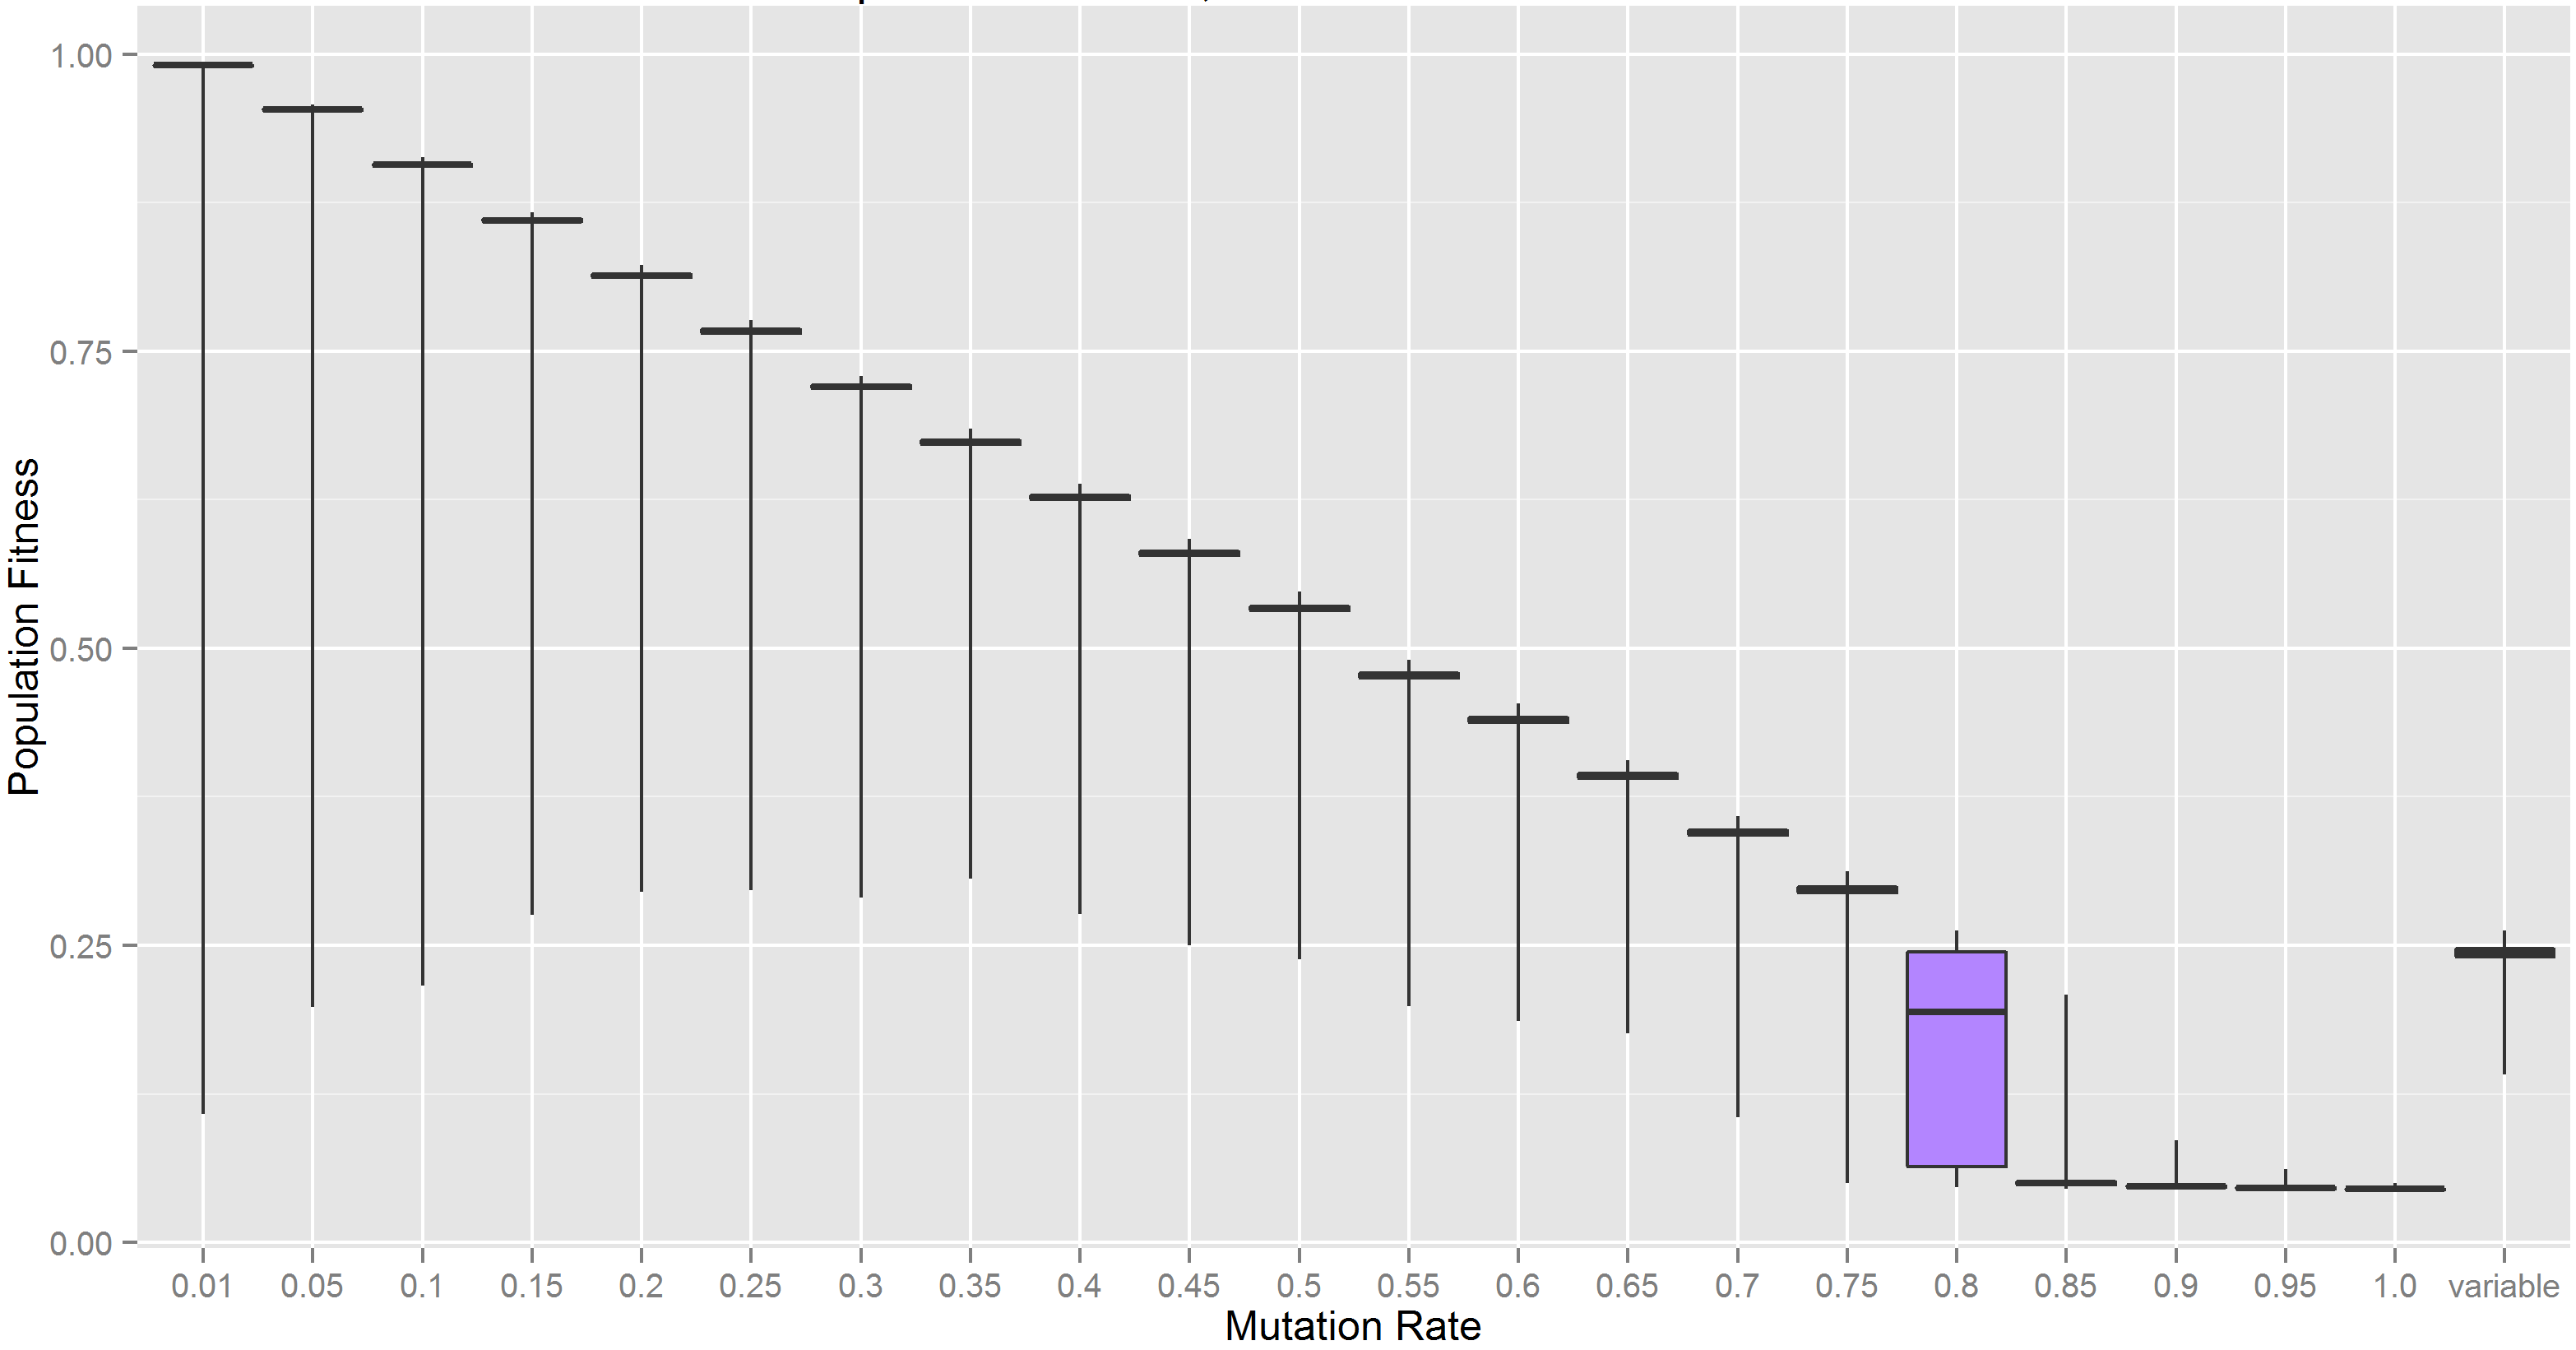
\includegraphics[width=0.50\textwidth]{fitness_all_mutation_14q.png}
\vspace{-18pt}
\caption{Population Fitness, All Mutation Rates, 14-Queens}
\label{fig:fitness_all_mutation_14}
\end{figure}



\subsection{Why Not Fixed Mutation?}
Variable adaptive mutation gives a distinct advantage over traditional genetic algorithms because of the optimization of a specific parameter \cite{hesser1991towards,ye2010some}. By using a variable mutation rate, replacing the mutation parameter with a chromosome similarity, better results can be gleaned while knowing less about the problem landscape or the best static mutation rate to use. Our results show that our variable adaptive mutation approach can perform better than static mutation values for large problems. As the problem becomes too large and unmanageable for traditional deterministic methods, our methodology can still produce useful results. When examining larger problems, our results show that having \emph{a priori} knowledge about the best static mutation parameter still does not yield results as good as those generated from our adaptive mutation approach.

\section{Conclusions and Further Study Remarks}
We conclude that using our variable adaptive mutation rate approach yields better results than traditional GA using fixed mutation rates in larger problems. Further research into adjusting the simplified chromosome similarity parameter that replaces mutation rate may yield even better results. Fixed values were used for our chromosome similarity parameter, and varying this parameter may yield more information about how variable adaptive mutation using our approach can be tuned further towards different problem landscapes.

Exploring our variable mutation rate approach in other NP-Complete combinatorial and optimization problems such as the Traveling Salesman Problem or Constraint Satisfaction Problem may show that our approach is valid for a multitude of problems. We conjecture that this is likely since other adaptive mutation methodologies have yielded performance improvements in various problem domains.

Conducting a multivariate analysis and sensitivity analysis of tuning other parameters in conjunction with the variable adaptive mutation rate may yield further performance improvements. For example, variable population size based on the amount of inbreeding may yield different results. This conjecture is based on the fact that with higher mutation rates, survival fitness decreases, resulting in population shrinkage. Coupling the population size with the mutation rate and patterns of fitness in the GA population may yield a new avenue for future study.


% trigger a \newpage just before the given reference
% number - used to balance the columns on the last page
% adjust value as needed - may need to be readjusted if
% the document is modified later
%\IEEEtriggeratref{8}
% The "triggered" command can be changed if desired:
%\IEEEtriggercmd{\enlargethispage{-5in}}

% references section
% NOTE: BibTeX documentation can be easily obtained at:
% http://www.ctan.org/tex-archive/biblio/bibtex/contrib/doc/

% can use a bibliography generated by BibTeX as a .bbl file
% standard IEEE bibliography style from:
% http://www.ctan.org/tex-archive/macros/latex/contrib/supported/IEEEtran/testflow/bibtex
%\bibliographystyle{IEEEtran.bst}
% argument is your BibTeX string definitions and bibliography database(s)
%\bibliography{IEEEabrv,../bib/paper}
%
% <OR> manually copy in the resultant .bbl file
% set second argument of \begin to the number of references
% (used to reserve space for the reference number labels box)


\def\V{\rm vol.~}
\def\N{no.~}
\def\pp{pp.~}
\def\Pot{\it Proc. }
\def\IJCNN{\it International Joint Conference on Neural Networks\rm }
\def\ACC{\it American Control Conference\rm }
\def\SMC{\it IEEE Trans. Systems\rm , \it Man\rm , and \it Cybernetics\rm }

\def\handb{ \it Handbook of Intelligent Control: Neural\rm , \it
    Fuzzy\rm , \it and Adaptive Approaches \rm }

\begin{thebibliography}{22}
\bibitem{cit:1} A. Krogh, J. Hertz and R.G. Palmer,
        {\it Introduction to the Theory of Neural Computation.}
        Addison-Wesley, Redwook City, CA, 1991.

\bibitem{cit:2} D. Marr and T. Poggio, ``Cooperative computation of stereo disparity,"
        {\it Science}, vol. 195, pp. 283-328, 1977.

\bibitem{cit:3} A.L. Yuille and D. Geiger,
        {\it The Handbook of Brain Theory and Neural Networks.}
        Chapter Winner-Take-All Networks, pp. 1228-1231, The MIT Press, 2 edition, 2002.

\bibitem{cit:4} W. Maass, ``Neural computation with winner-take-all as the only nonlinear
operation,"
        {\it Advances in Neural Information Processing Systems}, vol. 12, 2000.

\bibitem{cit:5} W. Maass, ``On the computational power of
winner-take-all,"
        {\it Neural Computation}, vol. 12, pp. 2519-2535, 2000.

\bibitem{cit:6} W.J. Wolfe, D. Mathis, C. Anderson, J. Rothman, M. Gottler, G. Brady, R. Walker, G. Duane and G. Alaghband, ``K-winner networks,"
        {\it IEEE Transactions on Neural Networks}, vol. 2, pp. 310-315, Mar. 1991.

\bibitem{cit:7} J. Wang, ``Analogue winner-take-all neural networks for determining maximum and minimum signals,"
        {\it Int. J. Electronics}, vol. 77, no. 3, pp. 355-367, 1994.

\bibitem{cit:8} K. Urahama and T. Nagao, ``K-winners-take-all ciucuit with O(N) complexity,"
        {\it IEEE Transactions on Neural Networks}, vol. 6, pp. 776-778, May. 1995.

\bibitem{cit:9} B. Sekerkiran and U. Cilingiroglu, ``A CMOS k-winners-take-all circuit with O(N) complexity,"
        {\it IEEE Transactions on Circuits and Systems}, vol. 46, no. 1, Jan. 1999.

\bibitem{cit:10} Jayadeva and S.A. Rahman, ``A neural network with O(N) neurons for ranking N numbers in O(1/N) times,"
        {\it IEEE Transactions on Circuits and Systems I}, vol. 51, no. 10, Oct. 2004.

\bibitem{cit:11} J. Yen, J. Guo and H. Chen, ``A new k-winners-take-all neural network and its array architecture,"
        {\it IEEE Transactions on Neural networks}, vol. 9, no. 5. pp. 901-912, Sept. 1998.

\bibitem{cit:12} B.D. Calvert and C.A. Marinov, ``Another k-winners-take-all analog neural network,"
        {\it IEEE Transactions on Neural Networks}, vol. 11, no. 4, pp. 829-838, Jul. 2000.

\bibitem{cit:13} C.A. Marinov and B.D. Calvert, ``Performance analysis for a k-winners-take-all analog neural network: basic theory,"
        {\it IEEE Transactions on Neural Networks}, vol. 14, no. 4, pp. 766-780, Jul. 2003.

\bibitem{cit:29} C.A. Marinov and J.J. Hopfield, ``Stable computational dynamics for a class of circuits with O(N) interconnections capable of KWTA and rand extractions,"
        {\it IEEE Transactions on Circuits and Systems}, vol. 52, no. 5, pp. 949-959, May 2005.

\bibitem{cit:14} D.W. Tank and J.J. Hopfield, ``Simple neural optimization networks: An A/D converter, signal decision circuit, and a linear programming circuit,"
        {\it IEEE Transactions on Circuits and Systems}, vol. 33, no. 5, pp. 533-541, 1986.

\bibitem{cit:15} J.J. Hopfield and D.W. Tank, ``Computing with neural circuits: A model,"
        {\it Science}, vol. 233, pp. 625-633, 1986.



\bibitem{cit:30} S.B. Liu and J. Wang, ``A simplified dual neural network for quadratic programming with its KWTA application,"
        {\it IEEE Transactions on Neural Networks}, vol. 17, no. 6, pp. 1500-1510, Nov 2006.



\bibitem{cit:16} M.P. Kennedy and L.O. Chua, ``Neural networks for nonlinear programming,"
        {\it IEEE Transactions on Circuits and Systems}, vol. 35, no. 5, pp. 554-562, May. 1988.

\bibitem{cit:17} S. Zhang and A.G. Constantinides, ``Lagrange programming neural networks,"
        {\it IEEE Transactions on Circuits and Systems II}, vol. 39, no. 7, pp. 441-452, Jul. 1992.

\bibitem{cit:18} J. Wang, ``A deterministic annealing neural network for convex programming,"
        {\it Neural Networks}, vol. 5, no. 4, pp. 962-971, 1994.

\bibitem{cit:19} Y. Xia, ``A new neural network for solving linear and quadratic programming problems,"
        {\it IEEE Transactions on Neural Networks}, vol. 7, no. 6, pp. 1544-1547, Nov. 1996.

\bibitem{cit:20} Y. Xia, G. Feng and J. Wang, ``A primal-dual neural network for online resolving constrained kinematic redundancy in robot motion control,"
        {\it IEEE Transactions on Systems, Man and Cybernetics}, vol. 35, no. 1, pp.54-64, Feb. 2005.

\bibitem{cit:21} Y. Xia and J. Wang, ``A dual neural network for kinematic control of redundant robot manipulators,"
        {\it IEEE Transactions on Systems, Man and Cybernetics}, vol. 31, no. 1, pp.147-154, Feb. 2001.

\bibitem{cit:22} Y. Zhang and J. Wang, ``A dual neural network for convex quadratic programming subject to linear equality and inequality constraints,"
        {\it Physics Letters A}, pp. 271-278, Jun. 2002.

\bibitem{cit:23} S. Boyd and L. Vandenbeghe,
        {\it Convex Optimization.}
        Cambridge University Press, Cambridge, UK. 2004.

\bibitem{cit:24} Y. Xia and J. Wang, ``Neural network for solving linear programming problems with bounded variables,"
        {\it IEEE Transactions on Neural Networks}, vol. 6, no. 2, pp. 515-519, 1995.

\bibitem{cit:25} Y. Xia, ``A new neural network for solving linear programming problems and its application,"
        {\it IEEE Transactions on Neural Networks}, vol. 7, no. 2, pp. 525-529, 1996.

\bibitem{cit:26} Y. Xia and J. Wang, ``A recurrent neural network for solving nonlinear convex programs subject to linear constraints,"
        {\it IEEE Transactions on Neural Networks}, vol. 16, no. 2, pp. 378-386, 2005.

\bibitem{cit:27} Y. Xia and J. Wang, ``A general projection neural network for solving monotone variational inequalities and related optimization problems,"
        {\it IEEE Transactions on Neural Networks}, vol. 15, no. 2, pp. 318-328, 2004.



\bibitem{cit:28} D.P. Bertsekas and J.N. Tsitsiklis,
        {\it Parallel and Distributed Computation: Numerical Methods.}
        Prentice-Hall, Englewood Cliffs, NJ, 1989.



\end{thebibliography}

% that's all folks
\end{document}
